%\documentclass[a0,portrait,boxedsections,final,25pt]{sciposter}
%\documentclass[a0,landscape,final,25pt,plainboxedsections]{sciposter}
%\documentclass[custom,landscape,final,25pt,plainboxedsections]{sciposter}
%\documentclass[custom,landscape,final,30pt,plainboxedsections]{sciposter}
\documentclass[custom,landscape,final,30pt,plainboxedsections]{sciposter-titleskipsmall}
\usepackage[numbers]{natbib}
\pdfcompresslevel=9
%\usepackage[tight]{subfigure}
%\usepackage{hyperref}
\usepackage{multicol}
\usepackage[american]{babel}
\usepackage[latin1]{inputenc}
\usepackage[T1]{fontenc}
\usepackage{ae}
\usepackage{aecompl}
\usepackage{xspace}
\usepackage[final]{graphicx}
\usepackage{wrapfig}
\usepackage{latexsym}
\usepackage{verbatim}
\usepackage{amsmath,amsfonts,amstext,amssymb,amsbsy,amsopn,amsthm,eucal}
\usepackage{wasysym}
\usepackage{dsfont}
\usepackage[normalem]{ulem}
\usepackage{overpic}
\renewcommand{\mastercapstartstyle}[1]{\textit{\textbf{#1}}}

\title{Computational Identification of structural RNAs using Infernal and Rfam}
\author{Eric Nawrocki(1), Ioanna Kalvari(2), Joanna Argasinska(2), Anton Petrov(2) and Sean Eddy(3)}
%\author{Eric Nawrocki}
\institute{1: National Center for Biotechnology Information, U.S. National Library of Medicine, Bethesda, MD 20894, USA. 2: European Molecular Biology Laboratory, European Bioinformatics Institute, Wellcome Trust Genome Campus, Hinxton, Cambridge CB10 1SD, UK. 3: Howard Hughes Medical Institute, FAS Center for Systems Biology, John A. Paulson School of Engineering and Applied Sciences, Harvard University, Cambridge, Massachusetts 02138, USA.}
%\institute{1: National Center for Biotechnology Information, U.S. National Library of Medicine, Bethesda, MD 20894, USA.}
%$^*$ {\tt davisf@janelia.hhmi.org}}
\email{nawrocke@ncbi.nlm.nih.gov}
\rightlogo[0.8]{figs/infernal-rfam-logos.pdf}
\leftlogo[1.0]{figs/nih-nlm-ncbi-hhmi-ebi-bbsrc.pdf}
\definecolor{mainCol}{rgb}{1,1,1}
\definecolor{BoxCol}{rgb}{0.95,0.95,1}
%\definecolor{BoxCol}{rgb}{0.1,0.5,0.5}
%\definecolor{BoxCol}{rgb}{0.1,0.5,0.5}
\definecolor{TextCol}{rgb}{0,0,0}
%\definecolor{SectionCol}{cmyk}{0.4,0.0,0.0,0.6}
\definecolor{SectionCol}{rgb}{0,0,0}
\setmargins[1in]
\begin{document}
\renewcommand{\titlesize}{\Huge}
\renewcommand{\authorsize}{\LARGE}
\renewcommand{\instsize}{\small}
\renewcommand{\sectionsize}{\large}
\maketitle

\setlength{\columnseprule}{0pt}
\begin{multicols}{3}

%%%%%%%%%%%%%%%
% Left column %
%%%%%%%%%%%%%%%

\section*{RNA genome annotation}
%\begin{Large}
Functional RNAs do not encode proteins, but rather function directly
as RNAs. Many of these RNAs form stable, evolutionarily conserved
three-dimensional structures that are crucial to their functions in
various fundamental cellular processes including protein synthesis,
gene expression, splicing, protein transport, and more. Despite their
importance, many genome annotation pipelines do not attempt to
annotate known structural RNAs, with the exception of transfer RNAs
(tRNA) and ribosomal RNAs (rRNA). The table below lists the number of
RNAs annotated in a sampling of published genomes:

\input{tables/tbl-genomes-nine}

\begin{comment}
Infernal includes several programs that are used in combination by
following four basic steps:

\bigskip
\begin{enumerate}
\item Build covariance models from alignments with \textt{cmbuild}.\\
\item Perform a simulation to determine E-value and filtering
  parameters with \texttt{cmcalibrate}.
\item Search target databases for putative homologs with \texttt{cmsearch}.
\item Create multiple alignments of putative homologs with \texttt{cmalign}.
\end{enumerate}

\begin{center}
\includegraphics[width=11.5in]{ismb2010/figs/ssu_list_and_seq2tree.png}
\end{center}
\end{comment}

\section*{Infernal and Rfam: tools for automated RNA genome annotation}
%\begin{Large}
Infernal is a software package for homology search and alignment of
RNAs using sequence-and-structure based family models called
covariance models (CMs). Rfam is a database that includes nearly 2000
CMs, each modeling a different functional RNA family. Using Rfam CMs,
Infernal can be used to annotate known RNAs in genome sequences.


%\section*{Faster searches using profile HMM filters}
\vspace{0.2in}

Because they model conserved structure as well as sequence, CM
searches can be more powerful than sequence-only based methods like
profile HMMs or BLAST. But they are also slower because of the higher
complexity of CM search algorithms.  To make searches faster, Infernal
v1.1 (available soon)
uses profile HMMs as prefilters to remove much of the database prior
to employing the CM. The filter pipeline used by the next, soon-to-be
released, version of Infernal is based on HMMER3~\cite{hmmer} and is
summarized below:


\begin{center}
\begin{small}
\begin{tabular}{rllllrr}
       &                             &          &          &       & HMMER3       & Infernal \\
filter &                             &          & model    & DP    & P-value      & P-value        \\
stage  & filter algorithm            & model    & locality & bands & threshold    & threshold      \\ \hline
1      & ungapped Viterbi (SSV)      & HMM      & local    & none  & 0.02         & 0.35           \\
2      & Viterbi                     & HMM      & local    & none  & 0.001        & 0.15           \\
3      & Forward                     & HMM      & local    & none  & 0.00001      & 0.003          \\
4      & Forward                     & HMM      & global   & none  & N/A          & 0.003          \\
5      & Forward/Backward            & HMM      & global   & none  & N/A          & 0.003          \\
       & (envelope definition)       &          &          &       &              &                \\
6      & CYK                         & CM       & local    & HMM-derived\cite{Brown00,Nawrocki09b} &  N/A   & 0.0001 \\
       & Inside                      & CM       & local    & HMM-derived\cite{Brown00,Nawrocki09b} &  N/A   & final  \\
\end{tabular}
\end{small}
\end{center}

\begin{comment}
\begin{center}
\begin{small}
\begin{tabular}{llllll}
     &              &                             &                               & already       & necessary for \\
     & Infernal     &                             &                               & computed      & annotating your \\
step & program      & input                       & output                        & in Rfam?      & favorite genome? \\ \hline
& & & & & \\
1    & cmbuild      & multiple sequence           & CM of                         & yes, for      & no, use  \\
     & and          & alignment of family X       & family X                      & 1446 families & Rfam CMs \\
     & cmcalibrate  & with structure              &                               &               & \\
& & & & & \\
%cmcalibrate  & CM of family X              & CM of                         & yes, for      & no, use \\
%             &                             & family X                      & 1446 families & Rfam CMs \\
%             &                             & w/E-value                     &               & \\
%             &                             & statistics                    &               & \\
%& & & & & \\
2    & cmsearch     & CM of family X              & putative                      & yes, for      & {\bf yes} \\
     &              & and target                  & homologs in                   & the RFAMSEQ   & \\
     &              & sequence file               & target                        & database      & \\
& & & & & \\
3    & cmalign      & CM of family X              & multiple                      & yes, for      & optional \\
     &              & and putative                & alignment                     & the RFAMSEQ   & \\
     &              & homologs                    & of homlogs                    & database      & \\
\end{tabular}
\end{small}
\end{center}
\end{comment}

\columnbreak
%%%%%%%%%%%%%%%%%
% Middle column %
%%%%%%%%%%%%%%%%%

\section*{The advantage of modeling structure} 
The conserved secondary structure of RNAs offers a
statistical signal that can be harnessed when searching
databases for homologs using CMs. In
Figure~\ref{fig:seqstructprofiles} below, the amount of information,
measured in \emph{bits}, inherent in a sequence-only profile (14
bits) and a sequence-and-structure profile (17 bits) is shown for a
toy example of an RNA family. We expect a match to a sequence-only
profile for this family once in every $2^{14}=4096$ random
nucleotides.  Additionally modeling structure with a
sequence-and-structure based profile (like a CM) reduces this
probability 8-fold, to once every every $2^{17}=32,764$ random
nucleotides.

\begin{footnotesize}
\begin{figure}
\center{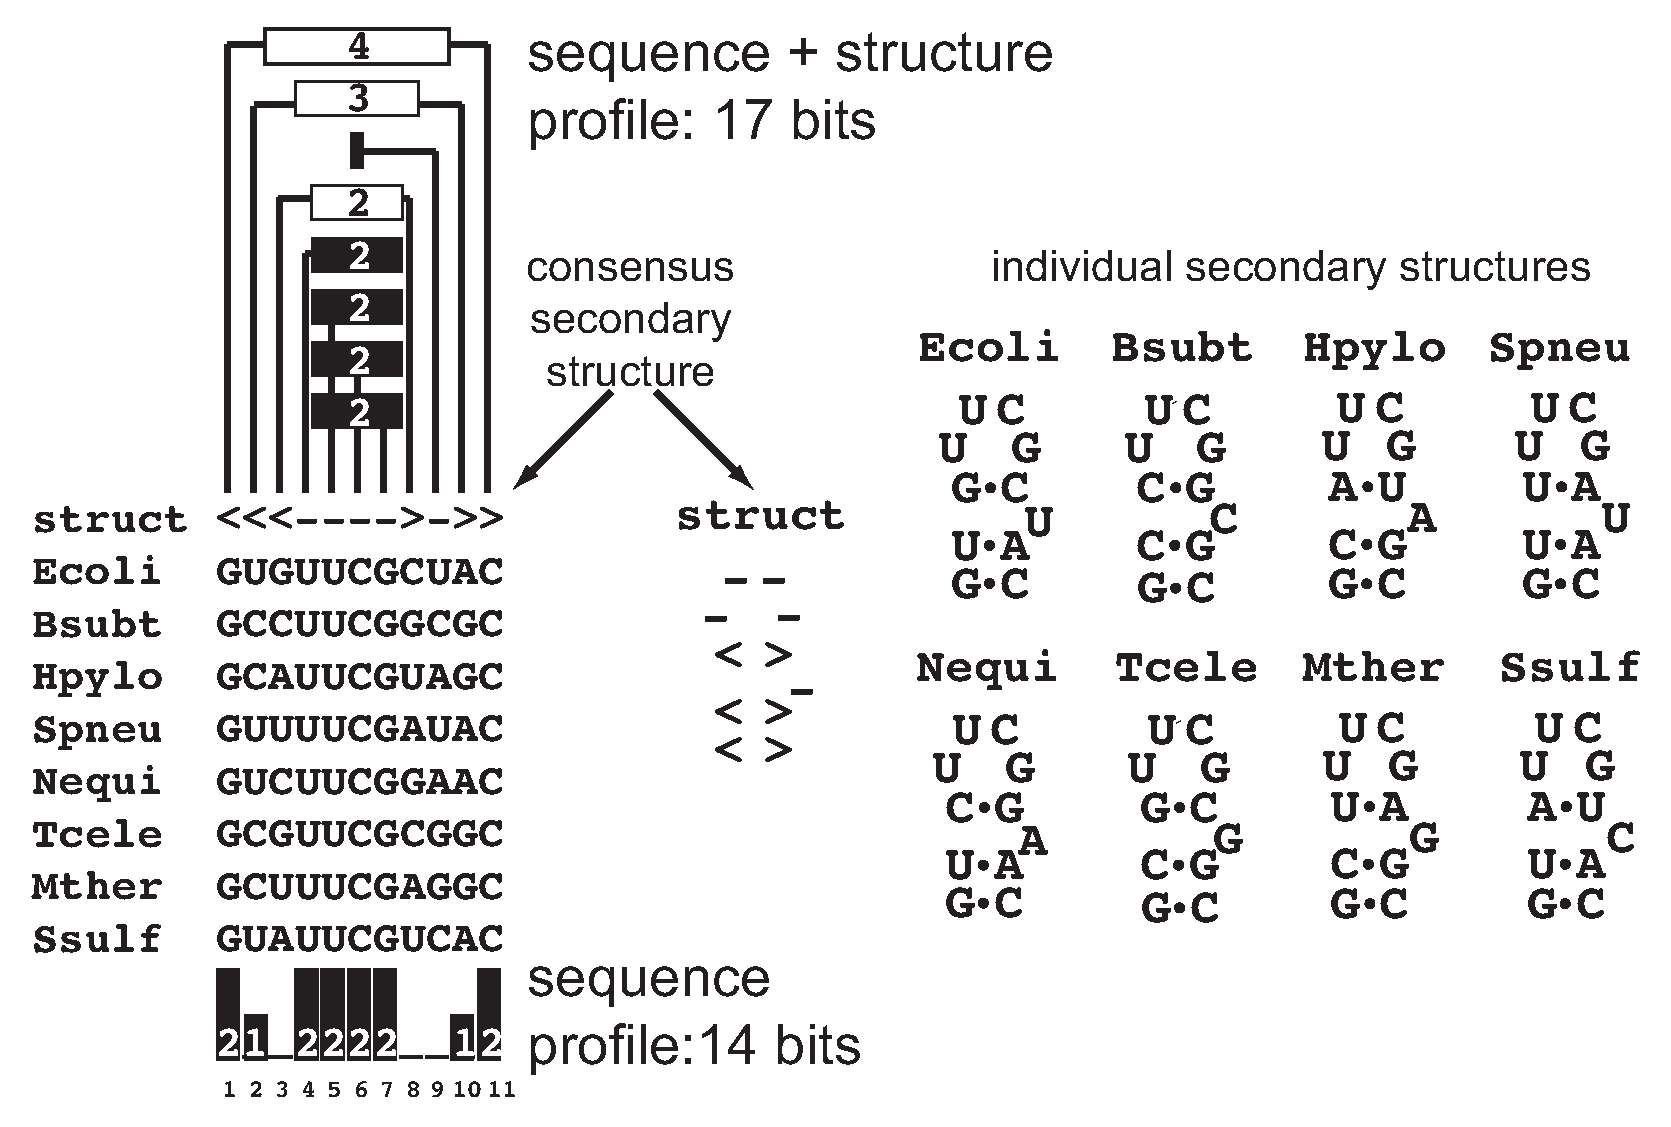
\includegraphics[width=11in]{figs/seqstructprofiles}}
\caption{Information in a sequence-only versus a sequence and
  structure profile. 
%The eight sequence alignment for a fabricated RNA
%  family used to build both of the profiles is on the left. 
%  The {\tt struct} line denotes the consensus secondary structure of the
%  family, with basepaired columns indicated by matching nested {\tt <}
%  and {\tt >} characters and connected by lines at top of figure. 
% The
%  structure is ignored by the sequence-only profile but used in the
%  sequence and structure profile to define dependencies between
%  basepaired columns. 
%  The eight individual secondary structures,
%  defined by imposing the consensus structure on each sequence, are
%  shown on the right. 
  Boxes with internal numbers at top and bottom of
  the alignment indicate the number of bits per position from the
  sequence (black), or per basepair from the structure (white).
  This figure is similar to one from \cite{Eddy06b} and 
  will appear in a chapter of an upcoming book from Humana Press.
}
\label{fig:seqstructprofiles}
\end{figure}
\end{footnotesize}

The amount of additional information gained from structure varies
widely for real RNA families, as shown for about 100 families in
Figure~\ref{fig:avgscores} below. 
%Some RNAs, like tRNA, include about
%as much information in their structure as in their sequence, while for
%others, the increase is relatively modest. 
Note that for most families, modeling structure contributes at least
10 additional bits of information, which corresponds to lowering the
expected chance of a false positive in a random database (i.e. the
E-value of a database hit) by three orders of magnitude
($2^{10}=1024$).

\begin{footnotesize}
\begin{figure}
\center{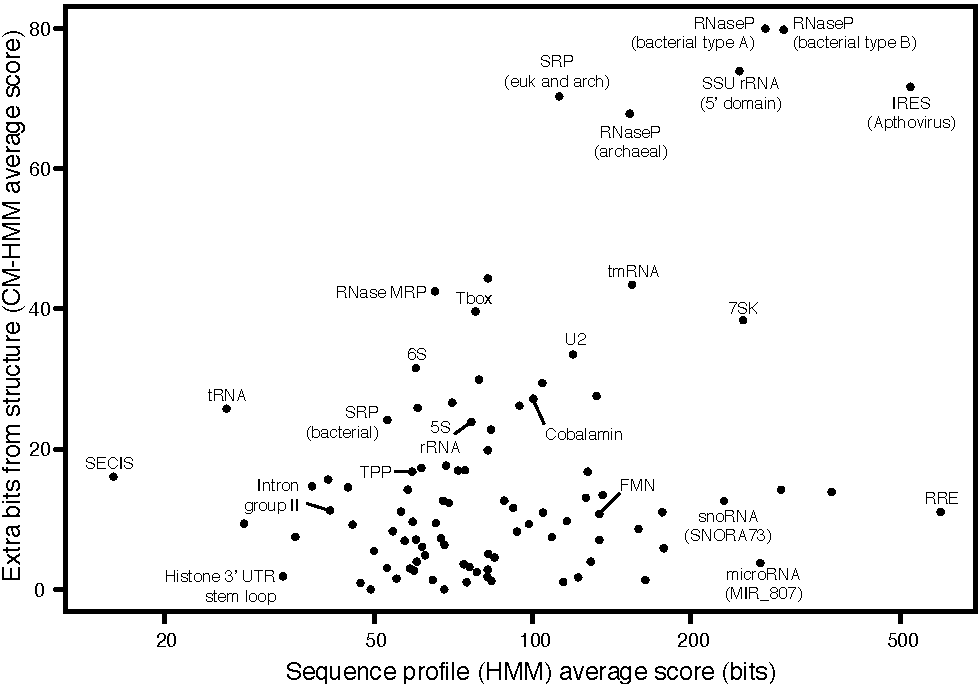
\includegraphics[width=11in]{figs/avgscores}}
\caption{Additional information (in bits) gained by sequence and
  structure profiles (CMs) versus sequence-only profiles (HMMs) for
  various RNA families.  
%  Sequence and structure profiles are most
%  advantageous for families with less primary sequence information
%  (towards left) and more secondary structure information (towards
%  top), so Rfam families that gain the most from including secondary
%  structure terms in a homology search are those toward the upper left
%  quadrant. 
  Data shown for the 95 Rfam release 9.1 families
  with 50 or more sequences in the \emph{seed} alignment. For each
  family, the seed alignment was used to build two profile models, a
  CM and a profile HMM. From each model, 10,000 sequences were
  generated and scored, and the average score per sampled sequence was
  calculated. Infernal version 1.0 was used for all steps.
  This figure will appear in a chapter of an upcoming book from Humana Press.
%  Several of the
%  outlying points are labeled by the name of RNA family as given by
%  Rfam. Note that the x-axis is drawn on a log scale. Models were
%  built and sequences were generated and scored using Infernal version
%  1.0 programs cmbuild, cmemit and cmalign.}
}
\label{fig:avgscores}
\end{figure}
\end{footnotesize}

%%%%%%%%%%%%%%%%%%%%%%%%%%%%%%%%%%%%%%%%%%%%%%%%%%%%%%%%%%%%%%%%%%%%%%%%
% TABLE that includes --rfam option; commented out.
\begin{comment}
\begin{center}
\begin{small}
\begin{tabular}{|r|l|l|l|r|r|r|}
\hline
       &                             &          &          & {\tt nhmmer} & {\tt cmsearch} & {\tt cmsearch} \\
       &                             &          &          & (default)    & (default)      & {\tt --rfam}   \\
       &                             &          & model    & P-value      & P-value        & P-value        \\
       & filter algorithm            & model    & locality & threshold    & threshold      & threshold      \\ \hline
1      & multi-segment Viterbi       & HMM      & local    & 0.02         & 0.40           & 0.02           \\
       & (MSV)                       &          &          &              &                &                \\
2      & Viterbi                     & HMM      & local    & 0.001        & 0.15           & 0.008          \\
3      & Forward                     & HMM      & local    & 0.00001      & 0.02           & 0.001          \\
4      & Forward                     & HMM      & global   & N/A          & 0.02           & 0.001          \\
5      & Forward/Backward            & HMM      & global   & N/A          & 0.02           & 0.001          \\
5      & (envelope definition)       &          &          &              &                &                \\
6      & CYK                         & CM       & local    & N/A          & 0.00005        & 0.00005        \\ \hline
\end{tabular}
\end{small}
\end{center}
\end{comment}
%%%%%%%%%%%%%%%%%%%%%%%%%%%%%%%%%%%%%%%%%%%%%%%%%%%%%%%%%%%%%%%%%%%%%%%%

\bibliographystyle{unsrtnat}
\begin{tiny}
\bibliography{poster}
\end{tiny}

\columnbreak
%%%%%%%%%%%%%%%%
% Right column %
%%%%%%%%%%%%%%%%

\section*{Example annotation of an archaeal genome}

As an illustrative example, I used Infernal 1.1 and Rfam CMs to annotate
RNAs in the genome of the methanogenic archaeon
\emph{Methanobrevibacter ruminantium} which lives in the stomachs of
ruminant mammals such as cows. The results of searching the 102 CMs for
Rfam families with representatives in archaea against the genome are
given below.  Infernal finds 175 hits with E-values below $0.0098$ ($1/102$)
from 12 different families. The GenBank annotation includes 
66 RNAs from 4 families.

\input{tables/tbl-mrum.tex}

\vspace{0.5in}

\section*{Comparing Infernal with family-specific tools}

A CM can be built and used to search for any RNA family with Infernal.
In contrast to this general approach, many family-specific methods for
RNA annotation have been developed including some that use
family-specific filtering heuristics prior to running CMs (e.g. 
tRNAscan-SE\cite{LoweEddy97} for tRNA, Bcheck\cite{Yusuf10} for RNase
P RNA and SRPscan\cite{Regalia02} for SRP RNA). Others do not use CMs
at all, such as Aragorn for tRNA and tmRNA and RNAmmer\cite{Lagesen07}
for ribosomal RNAs. As the comparison in Table~\ref{tbl:compare} below
shows, the sensitivity of Infernal and these methods is similar,
and the speeds are comparable in many cases:

\input{tables/tbl-compare.tex}

\end{multicols}

\end{document}
